\documentclass[varwidth,border=10pt]{standalone}
\usepackage{subcaption}
\usepackage[labelformat=parens,labelsep=quad, skip=3pt]{caption}
\usepackage{graphicx}
\begin{document}
\begin{figure}
\centering
\begin{subfigure}{6cm}
\centering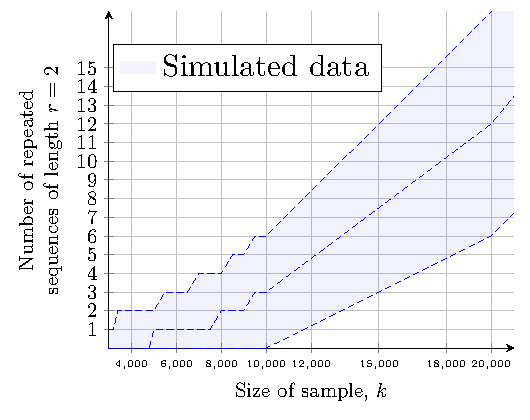
\includegraphics[width=5cm,page=1]{SubFigures.pdf}
\caption{Simulations, $k\in[3000,21000]$}
\end{subfigure}%
\begin{subfigure}{6cm}
\centering\includegraphics[width=5cm,page=2]{SubFigures.pdf}
\caption{Simulations, $k\in[3000,50000]$}
\end{subfigure}\vspace{10pt}
 
\begin{subfigure}{6cm}
\centering\includegraphics[width=5cm,page=4]{SubFigures.pdf}
\caption{Lower theoretical limit, $E_L$}
\end{subfigure}%
\begin{subfigure}{6cm}
\centering\includegraphics[width=5cm,page=3]{SubFigures.pdf}
\caption{Upper theoretical limit, $E_U$}
\end{subfigure}
\end{figure}
\end{document}
